\documentclass{beamer}

\usepackage[english]{babel}
\usepackage[utf8x]{inputenc}

\mode<presentation>
{
  \usetheme{default}
  \usecolortheme{default}
  \usefonttheme{default}
  \setbeamertemplate{caption}[numbered]
}

\usepackage{graphicx}
\usepackage{booktabs}
\usepackage{hyperref}
\usepackage{quantikz}
\usepackage{quiver}
\usepackage{mathtools}
% \usetikzlibrary{decorations.pathreplacing,calc}
\usetikzlibrary{shapes.geometric}
\usetikzlibrary{positioning,decorations.pathmorphing}

\newcommand{\Grid}{\textsf{Grid}}
\newcommand{\CGrid}{\textsf{CGrid}}
\newcommand{\LO}{\textsf{LO}}
\newcommand{\LOCC}{\textsf{LOCC}}
\newcommand{\CC}{\textsf{CC}}
\newcommand{\LU}{\textsf{LU}}
\newcommand{\LC}{\textsf{LC}}

\newtheorem{observation}{Observation}
\newtheorem{conjecture}{Conjecture}
\newtheorem{justification}{Justification}

\title{On the Universality of Comparability Grids for Measurement-Based Quantum Computation}
\author{Ryan Y. Batubara\\Advisor: Professor Daniel Grier}
\institute{UCSD\\[2\baselineskip]Mathematics Undergraduate Honors Presentation}
\date{February 13, 2026}

\begin{document}

\begin{frame}
  \titlepage
\end{frame}

\section{Background}

% \begin{frame}{The Circuit Model of Quantum Computation}

% Dirac notation: $\ket{0} = \begin{bmatrix} 1 \\ 0 \end{bmatrix}$, $\ket{1} = \begin{bmatrix} 0 \\ 1 \end{bmatrix}$.

% \vspace{0.5cm}

% \begin{center}

% \begin{tikzpicture}[remember picture]
% \node (C) [inner sep=0pt, outer sep=0pt] {
% \begin{quantikz}[row sep=0.55cm, column sep=0.45cm]
% \lstick{$\ket{\psi_1}$} & \gate{U_1} & \meter{} \\
% \lstick{$\ket{\psi_2}$} & \gate{U_2} & \meter{}
% \end{quantikz}
% };
% \end{tikzpicture}

% \begin{tikzpicture}[remember picture,overlay]
% \coordinate (NW) at ($(C.north west)$);
% \coordinate (NE) at ($(C.north east)$);
% \coordinate (SW) at ($(C.south west)$);
% \coordinate (SE) at ($(C.south east)$);

% \only<2->{%
% \draw[decorate,decoration={brace,amplitude=5pt},thick]
%   ($(SW)+(-0.2,0)$) -- ($(NW)+(-0.2,0)$)
%   node[midway,xshift=-1cm,align=left,text width=5.6cm]
%   {\textbf<2->{qubit\\}
%    $\ket{\psi}\in\mathbb{C}^2, $\\
%    $\ket{\psi}=\alpha\ket{0}+\beta\ket{1}, $\\
%    $|\alpha|^2+|\beta|^2=1$.};
% }

% \only<3->{%
% \draw[decorate,decoration={brace,amplitude=5pt,mirror},thick]
%   ($(SW)+(+1,-0.2)$) -- ($(SE)+(-1.1,-0.2)$)
%   node[midway,yshift=-0.95cm,align=left,text width=4cm]
%   {\textbf<3->{gate}\\
%    $U\in\mathbb{C}^{2\times 2}$\\
%   $U^\dagger U=I$ (unitary)};
% }

% \only<4->{%
% \draw[decorate,decoration={brace,amplitude=5pt,mirror},thick]
%   ($(SE)+(0.2,0)$) -- ($(NE)+(0.2,0)$)
%   node[midway,xshift=4cm,align=left,text width=6.2cm]
%   {\textbf<4->{measurement}\\
%    $b \in \{\ket{0},\ket{1}\}$\\
%    $\Pr(b) = |\langle b\mid\psi\rangle|^2$.\\
%    Works for any \\orthonormal basis\\of $\mathbb{C}^2$.};
% }
% \end{tikzpicture}

% \end{center}

% \vspace{1.5cm}

% \only<5->{%
% Composition between gates is by $\otimes$ to preserve linearity.
% }

% \end{frame}

\begin{frame}{Measurement-Based Quantum Computation (MBQC)}

\begin{tikzpicture}[remember picture]

\node (C) [inner sep=0pt, outer sep=0pt, anchor=west] at (0,0) {
\begin{quantikz}[row sep=0.45cm, column sep=0.45cm, wire types={q,n,q}]
\lstick{$\ket{0}$} & \gate[3]{C} & \meter{} \\
\lstick{$\vdots$}       &             & \vdots   \\
\lstick{$\ket{0}$} &             & \meter{}
\end{quantikz}
};

\only<2->{%
\draw[->, thick]
  ($(C.east)+(0.6,0)$) -- ($(C.east)+(3.2,0)$)
  coordinate[midway] (Amid);
}

\only<2->{%
\node[anchor=south] at ($(Amid)+(0,0.12)$)
{\scriptsize\textbf{MBQC}};
}

\node (B) [anchor=west] at ($(C.east)+(3.5,0)$) {
\only<3->{%
\begin{minipage}{0.4\linewidth}
\begin{itemize}\small
\item Single-qubit measurements on a
\item "resource state"
\item <4-> Excluding resource state, done in constant depth.
\end{itemize}
\end{minipage}
}
};
\end{tikzpicture}

\end{frame}

\begin{frame}{Example Resource State: Graph State}

Let $G = (V,E)$ be a graph. The \textbf{graph state} $\ket{G}$ has 
\begin{itemize}
    \item For every $v \in V$, prepare a qubit $\ket+ = H \ket0$.
    \item For every $e = (u,v) \in E$, apply $CZ$ on qubits of $u$ and $v$.
\end{itemize}

\vspace{0.5cm}

\only<2->{%
\makebox[\textwidth][c]{%
\begin{minipage}{0.3\textwidth}
\centering
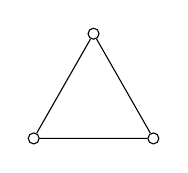
\begin{tikzpicture}[scale=0.95, every node/.style={circle,draw,inner sep=1.4pt}]
\node (a) at (0,0.9) {};
\node (b) at (-0.8,-0.5) {};
\node (c) at (0.8,-0.5) {};
\draw (a)--(b)--(c)--(a);
\end{tikzpicture}
\end{minipage}
\hspace{0.4cm}
\begin{minipage}{0.3\textwidth}
\centering
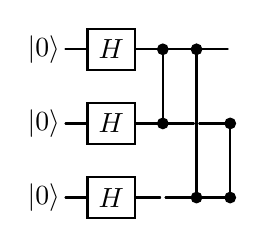
\begin{tikzpicture}
\node [inner sep=0pt, outer sep=0pt] {
\begin{quantikz}[row sep=0.42cm, column sep=0.28cm, cells={inner sep=1pt}]
\lstick{$\ket{0}$} & \gate{H} & \ctrl{1}  & \ctrl{2}  & \qw      \\
\lstick{$\ket{0}$} & \gate{H} & \ctrl{-1} & \qw       & \ctrl{1} \\
\lstick{$\ket{0}$} & \gate{H} & \qw       & \ctrl{-2} & \ctrl{-1}
\end{quantikz}
};
\end{tikzpicture}
\end{minipage}
}%
}

\end{frame}

\begin{frame}{Grid Graph State}

Let $\Grid_{m \times n}$ be the grid graph with $m$ rows and $n$ columns. \\
Let $\ket{\Grid_{m \times n}}$ be its graph state. 

\vspace{0.5cm}

\only<2->{Example: $\ket{\Grid_{2 \times 3}}$.}

\vspace{0.5cm}

\only<2->{%
\makebox[\textwidth][c]{%
\begin{minipage}{0.3\textwidth}
\centering
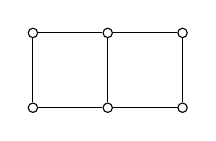
\begin{tikzpicture}[scale=0.95, every node/.style={circle,draw,inner sep=1.2pt}]
\node (a1) at (0,1) {};
\node (a2) at (1,1) {};
\node (a3) at (2,1) {};
\node (b1) at (0,0) {};
\node (b2) at (1,0) {};
\node (b3) at (2,0) {};
\foreach \u/\v in {a1/a2,a2/a3,b1/b2,b2/b3,a1/b1,a2/b2,a3/b3} \draw (\u)--(\v);
\end{tikzpicture}
\end{minipage}%
\hspace{0.35cm}%
\begin{minipage}{0.3\textwidth}
\centering
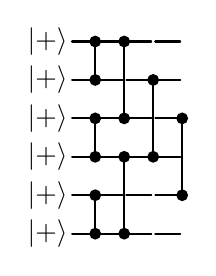
\begin{tikzpicture}
\node (Cgrid) [inner sep=0pt, outer sep=0pt] {
\begin{quantikz}[row sep=0.34cm, column sep=0.22cm, cells={inner sep=0.8pt}]
\lstick{$\ket{+}$} & \ctrl{1}  & \ctrl{2}  & \qw       & \qw       \\
\lstick{$\ket{+}$} & \ctrl{-1} & \qw       & \ctrl{2}  & \qw       \\
\lstick{$\ket{+}$} & \ctrl{1}  & \ctrl{-2} & \qw       & \ctrl{2}  \\
\lstick{$\ket{+}$} & \ctrl{-1} & \ctrl{2}  & \ctrl{-2} & \qw       \\
\lstick{$\ket{+}$} & \ctrl{1}  & \qw       & \qw       & \ctrl{-2} \\
\lstick{$\ket{+}$} & \ctrl{-1} & \ctrl{-2} & \qw       & \qw       
\end{quantikz}
};
\end{tikzpicture}
\end{minipage}%
}%
}

\end{frame}

\begin{frame}{Universal Resource, Informally}

\begin{definition}
Let $\LO$ denote local operations, i.e. single qubit unitaries and measurements. Let $\CC$ denote classical communication.
\end{definition}

\begin{definition}<2->
Let $\Psi$ be a family of resource states. $\Psi$ is a \textbf{universal resource} for MBQC if for every $U \in SU(2^n)$, $\forall n \in \mathbb{N}$, there is a sequence of $\LOCC$ and some resource state $\ket\psi \in \Psi$, such that 
\begin{align}
    \ket{\psi} \xrightarrow{\LOCC} U \ket{0^n}
\end{align}
\only<3->{%
In other words, we can ``simulate any state'' using $\LOCC$ and a resource state from $\Psi$.
}
\end{definition}

\end{frame}

\begin{frame}{Grid is a Universal Resource}

\begin{theorem}
$\{\Grid_{1 \times i}\}_{i\in \mathbb{N}}$ (The lines) are a 1-qubit universal resource for MBQC.
\end{theorem}

\begin{lemma}[Euler decomposition]
Every single-qubit unitary can be expressed (up to global phase) as the product
\begin{align}
    R_z(\theta_3)R_x(\theta_2)R_z(\theta_1)
\end{align}
for some $\theta_1, \theta_2, \theta_3 \in [0,2\pi]$.
\end{lemma}

\begin{lemma}
$R_x(\theta) = H R_z(\theta) H$, for all $\theta \in [0,2\pi]$.
\end{lemma}

\end{frame}

\begin{frame}{Grid is a Universal Resource cont'd}

\begin{proof}[Informal proof.]
\vspace{-0.8cm}
\begin{align}
\begin{quantikz}[row sep=0.2cm, column sep=0.2cm]
\lstick{$\ket{\phi}$} & \ctrl{1}  & \gate{R_z(\theta)} & \gate{H} & \meter{} \\
\lstick{$\ket{+}$}    & \ctrl{-1} & \qw      &          &
\end{quantikz}
\;=\;
\begin{quantikz}[row sep=0.2cm, column sep=0.2cm]
\lstick{$\ket{+}$}              & \ctrl{1}  & \meter{} \\
\lstick{$HR_z{\theta}\ket\phi$} & \targ{}   & \qw
\end{quantikz}
\end{align}
\only<2->{%
If we measure $0$, we get $HR_z(\theta)\ket\phi$ in the second register. If we measure $1$, we get $XH_z(\theta)\ket\phi$. Thus given the right measurements we can apply any 1-qubit gate by repeating the construction:
}
\only<3->{%
\begin{center}
\begin{quantikz}[row sep=0.1cm, column sep=0.1cm]
\lstick{$\ket{\phi}$} & \ctrl{1}  & \gate{R_z(\theta_1)} & \gate{H} & \meter{} \\
\lstick{$\ket{+}$}    & \ctrl{-1} & \ctrl{1}      & \gate{R_z(\theta_2)} & \gate{H} & \meter{} \\
\lstick{$\ket{+}$}    & \qw       & \ctrl{-1}     & \qw & \qw & \qw & \qw \\
\end{quantikz}
\end{center}
}
\end{proof}

\end{frame}

\begin{frame}{Grid is a Universal Resource cont'd}

\begin{theorem}
Let $\Grid$ denote the family of all grid graphs. $\Grid$ is a universal resource for MBQC.
\end{theorem}

\begin{proof}
Similar to the proof for the line.
\end{proof}

\end{frame}

\begin{frame}{Comparability Grid}

\begin{definition}
Let $\CGrid_{m \times n}$ denote the $m$ rows, $n$ column \textbf{comparability grid}, which is an undirected graph $G = (V,E)$ with
\begin{align}
    V &= \{(i,j) \mid i \in [m], j \in [n]\} \\
    E &= \{ \{(i_1,j_1),(i_2,j_2)\} \mid (i_1,j_1),(i_2,j_2) \in V, i_2 \geq i_1, j_2 \geq j_1. \}
\end{align}  
i.e. the grid with partial order $\leq$ defining edges.
\end{definition}

\end{frame}

\begin{frame}{Comparability Grid Example}

Example: $\CGrid_{3 \times 3}$:

\vspace{0.5cm}

\centering
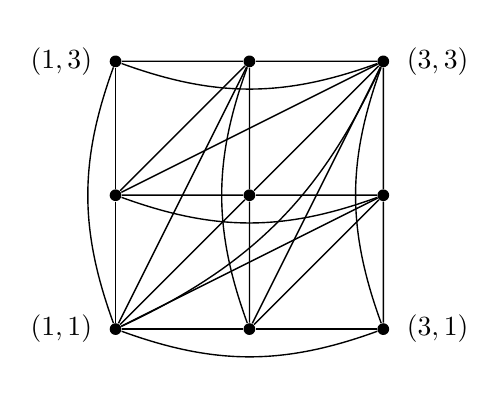
\begin{tikzpicture}[
  scale=1.7,
  every node/.style={circle, fill=black, inner sep=1.5pt},
  edge/.style={line width=0.5pt}
]
\node (v11) at (1,1) {};
\node (v12) at (1,2) {};
\node (v13) at (1,3) {};
\node (v21) at (2,1) {};
\node (v22) at (2,2) {};
\node (v23) at (2,3) {};
\node (v31) at (3,1) {};
\node (v32) at (3,2) {};
\node (v33) at (3,3) {};

\draw[edge] (v11) -- (v12);
\draw[edge] (v11) -- (v21);
\draw[edge] (v11) -- (v22);
\draw[edge] (v11) -- (v23);
\draw[edge] (v11) -- (v32);

\draw[edge] (v12) -- (v13);
\draw[edge] (v12) -- (v22);
\draw[edge] (v12) -- (v23);

\draw[edge] (v13) -- (v23);

\draw[edge] (v21) -- (v22);
\draw[edge] (v21) -- (v31);
\draw[edge] (v21) -- (v32);

\draw[edge] (v22) -- (v23);
\draw[edge] (v22) -- (v32);

\draw[edge] (v23) -- (v33);
\draw[edge] (v31) -- (v32);
\draw[edge] (v32) -- (v33);

\draw[edge] (v11) to[bend left=20] (v13);
\draw[edge] (v21) to[bend left=20] (v23);
\draw[edge] (v31) to[bend left=20] (v33);

\draw[edge] (v11) to[bend right=20] (v31);
\draw[edge] (v12) to[bend right=20] (v32);

\draw[edge] (v11) to[bend right=20] (v33);
\draw[edge] (v12) -- (v33);
\draw[edge] (v13) to[bend right=20] (v33);

\draw[edge] (v21) -- (v33);
\draw[edge] (v22) to (v33);

\node[draw=none, fill=none, inner sep=0pt, anchor=east] at ($(v13)+(-0.15,0)$) {$ (1,3)$};
\node[draw=none, fill=none, inner sep=0pt, anchor=west] at ($(v33)+(0.15,0)$) {$ (3,3)$};
\node[draw=none, fill=none, inner sep=0pt, anchor=east] at ($(v11)+(-0.15,0)$) {$ (1,1)$};
\node[draw=none, fill=none, inner sep=0pt, anchor=west] at ($(v31)+(0.15,0)$) {$ (3,1)$};
\end{tikzpicture}

\end{frame}

\section{Subgraphs of the Comparability Grid}

\begin{frame}{Proving Comparability Grid Universality}
Strategy: Embed $\Grid$ in $\CGrid$. Two ways to do this:

\[
\begin{tikzpicture}[x=1cm,y=1cm]
	\node[font=\Large] (cgrid) at (0,2.8) {$\CGrid$};
	\node[font=\Large] (grid) at (0,0) {$\Grid_{m \times n}$};
	\draw[->,thick,bend right=35] (cgrid) to node[midway,left=14pt,align=center,text width=3.8cm]
		{\only<2->{\textbf{Method 1}\\What grids can we get from vertex deletion?}} (grid);
	\draw[->,thick,bend right=35] (grid) to node[midway,right=14pt,align=center,text width=3.8cm]
		{\only<3->{\textbf{Method 2}\\How can we embed $\Grid_{m \times n}$ in $\CGrid$?}} (cgrid);
\end{tikzpicture}
\]

\end{frame}

\begin{frame}{$\Grid_{2 \times n}$ is a subgraph}

\begin{lemma}
For all $n \in \mathbb{N}$, $\Grid_{2 \times n}$ is a subgraph of a sufficiently large $\CGrid$.
\end{lemma}

\begin{proof}<2->

\begin{center}
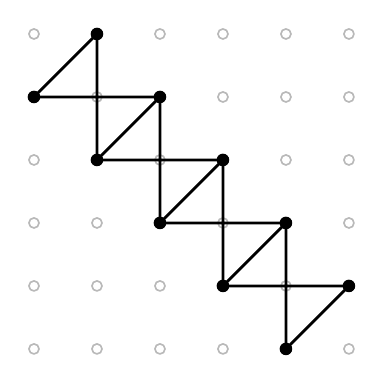
\begin{tikzpicture}[scale=0.8, line cap=round, line join=round]

\foreach \x in {0,...,5} {
    \foreach \y in {0,...,5} {
    \draw[gray!55, line width=0.6pt] (\x,\y) circle[radius=0.08];
    }
}

\draw[black, line width=1.0pt]
    (0,4)--(1,5)
    (1,5)--(1,4)
    (0,4)--(1,4)--(2,4)
    (1,4)--(1,3)
    (1,3)--(2,4)
    (1,3)--(2,3)--(2,4)
    (2,3)--(2,2)
    (2,3)--(3,3)
    (2,2)--(3,3)
    (2,2)--(3,2)--(3,3)
    (3,2)--(3,1)
    (3,2)--(4,2)
    (3,1)--(4,2)
    (3,1)--(4,1)--(4,2)
    (4,1)--(4,0)
    (4,1)--(5,1)
    (4,0)--(5,1);

\foreach \p in {(0,4),(1,5),(1,3),(2,4),(2,2),(3,3),(3,1),(4,2),(4,0),(5,1)}{
    \fill[black] \p circle[radius=0.10];
}

\end{tikzpicture}
\end{center}
\end{proof}

\end{frame}

\begin{frame}{Which grids are subgraphs?}

\begin{theorem}
$\Grid_{k \times n}$ is not a subgraph of any  $\CGrid$ for $k > 2$, $n > 2$.
\end{theorem}

\begin{proof}<2->
Using a computer, we enumerate all possible $9$ vertex subgraphs of $\CGrid$. No such subgraph is isomorphic to $\Grid_{3 \times 3}$.
\end{proof}

\end{frame}

\section{The Enumeration Algorithm}

\begin{frame}{Permutation Representation of Subgraphs}

\begin{lemma}
Any subgraph $H$ of $\CGrid$ with $|V(H)| = n$ can be uniquely identified as a permutation of $[n]$, denoted $\pi(H)$.
\end{lemma}

\begin{proof}<2->
Since $H \subseteq \CGrid$, each vertex has distinct $x,y$ coordinates. Name vertex $i$ by its rank sorting by $x + \frac{y}{n}$. Denote $\pi_i$ by the rank of vertex $i$ sorted by $y + \frac{x}{n}$. 

\vspace{0.5cm}

Conversely, given a permutation $\pi \in S_n$, construct vertices $(i, \pi_i)$ for $i=1,\dots,n$. This produces a subgraph of $\CGrid$ with $n$ vertices.

\vspace{0.5cm}

These are inverses of each other.
\end{proof}

\end{frame}

\begin{frame}{Example Permutation Representation}

\begin{example}
The following subgraph $H$ has $\pi(H) = (2,1,4,3)$, since the leftmost vertex is 2nd lowest in $y$ order, and so on.
\end{example}

\vspace{0.5cm}

\centering
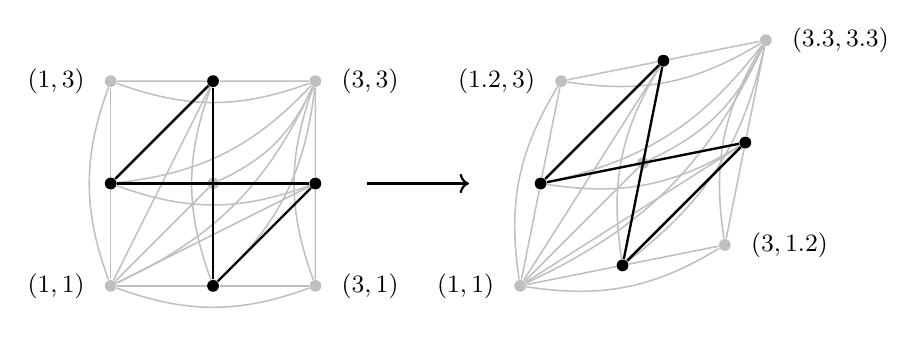
\begin{tikzpicture}[
    scale=1.3,
    dot/.style={circle, inner sep=1.5pt},
    faintdot/.style={dot, fill=black!25},
    sel/.style={dot, fill=black},
    faintedge/.style={line width=0.55pt, draw=black!25},
    seledge/.style={line width=0.85pt, draw=black},
    lab/.style={draw=none, fill=none, inner sep=0pt, font=\small},
]

\begin{scope}[xshift=0cm]
    % vertices
    \foreach \x in {1,2,3}{
    \foreach \y in {1,2,3}{
        \node[faintdot] (L-\x-\y) at (\x,\y) {};
    }
    }

    % select vertices (2,1), (1,2), (2,3), (3,2)
    \node[sel] (Lsel-2-1) at (2,1) {};
    \node[sel] (Lsel-1-2) at (1,2) {};
    \node[sel] (Lsel-2-3) at (2,3) {};
    \node[sel] (Lsel-3-2) at (3,2) {};

    % (faint) edges of CGrid_{3x3} copied from your reference
    \draw[faintedge] (L-1-1) -- (L-1-2);
    \draw[faintedge] (L-1-1) -- (L-2-1);
    \draw[faintedge] (L-1-1) -- (L-2-2);
    \draw[faintedge] (L-1-1) -- (L-2-3);
    \draw[faintedge] (L-1-1) -- (L-3-2);

    \draw[faintedge] (L-1-2) -- (L-1-3);
    \draw[faintedge] (L-1-2) -- (L-2-2);
    \draw[faintedge] (L-1-2) -- (L-2-3);

    \draw[faintedge] (L-1-3) -- (L-2-3);

    \draw[faintedge] (L-2-1) -- (L-2-2);
    \draw[faintedge] (L-2-1) -- (L-3-1);
    \draw[faintedge] (L-2-1) -- (L-3-2);

    \draw[faintedge] (L-2-2) -- (L-2-3);
    \draw[faintedge] (L-2-2) -- (L-3-2);

    \draw[faintedge] (L-2-3) -- (L-3-3);
    \draw[faintedge] (L-3-1) -- (L-3-2);
    \draw[faintedge] (L-3-2) -- (L-3-3);

    \draw[faintedge] (L-1-1) to[bend left=20] (L-1-3);
    \draw[faintedge] (L-2-1) to[bend left=20] (L-2-3);
    \draw[faintedge] (L-3-1) to[bend left=20] (L-3-3);

    \draw[faintedge] (L-1-1) to[bend right=20] (L-3-1);
    \draw[faintedge] (L-1-2) to[bend right=20] (L-3-2);

    \draw[faintedge] (L-1-1) to[bend right=20] (L-3-3);
    \draw[faintedge] (L-1-2) to[bend right=20] (L-3-3);
    \draw[faintedge] (L-1-3) to[bend right=20] (L-3-3);

    \draw[faintedge] (L-2-1) to[bend right=20] (L-3-3);
    \draw[faintedge] (L-2-2) to[bend right=20] (L-3-3);

    % chosen subgraph edges among the 4 chosen vertices
    \draw[seledge] (L-2-1) -- (L-3-2);
    \draw[seledge] (L-2-1) -- (L-2-3);
    \draw[seledge] (L-1-2) -- (L-3-2); 
    \draw[seledge] (L-1-2) -- (L-2-3);

    % corner labels (optional)
    \node[lab, anchor=east] at ($(L-1-1)+(-0.25,0)$) {$(1,1)$};
    \node[lab, anchor=east] at ($(L-1-3)+(-0.25,0)$) {$(1,3)$};
    \node[lab, anchor=west] at ($(L-3-1)+(0.25,0)$) {$(3,1)$};
    \node[lab, anchor=west] at ($(L-3-3)+(0.25,0)$) {$(3,3)$};
\end{scope}

% ---------------------------
% Arrow to sheared grid
% ---------------------------
\draw[->,thick] (3.5,2) to (4.5,2);

% ---------------------------
% Helper: middle grid (shear/shift y by 0.2*(x-1))
% (x,y) -> (x, y + 0.2*(x-1))
% ---------------------------
\begin{scope}[xshift=4cm]
    % vertices
    \foreach \x in {1,2,3}{
    \foreach \y in {1,2,3}{
        \pgfmathsetmacro{\dx}{0.2*(\y-1)} % shift x depending on y
        \pgfmathsetmacro{\dy}{0.2*(\x-1)} % shift y depending on x
        \node[faintdot] (M-\x-\y) at (\x+\dx,\y+\dy) {};
    }
    }

    % select vertices
    \node[sel] (Msel-2-1) at (2,1+0.2) {};
    \node[sel] (Msel-1-2) at (1+0.2,2) {};
    \node[sel] (Msel-2-3) at (2+0.4,3+0.2) {};
    \node[sel] (Msel-3-2) at (3+0.2,2+0.4) {};

    % faint edges: same adjacency, just using shifted coordinates
    \draw[faintedge] (M-1-1) -- (M-1-2);
    \draw[faintedge] (M-1-1) -- (M-2-1);
    \draw[faintedge] (M-1-1) -- (M-2-2);
    \draw[faintedge] (M-1-1) -- (M-2-3);
    \draw[faintedge] (M-1-1) -- (M-3-2);

    \draw[faintedge] (M-1-2) -- (M-1-3);
    \draw[faintedge] (M-1-2) -- (M-2-2);
    \draw[faintedge] (M-1-2) -- (M-2-3);

    \draw[faintedge] (M-1-3) -- (M-2-3);

    \draw[faintedge] (M-2-1) -- (M-2-2);
    \draw[faintedge] (M-2-1) -- (M-3-1);
    \draw[faintedge] (M-2-1) -- (M-3-2);

    \draw[faintedge] (M-2-2) -- (M-2-3);
    \draw[faintedge] (M-2-2) -- (M-3-2);

    \draw[faintedge] (M-2-3) -- (M-3-3);
    \draw[faintedge] (M-3-1) -- (M-3-2);
    \draw[faintedge] (M-3-2) -- (M-3-3);

    \draw[faintedge] (M-1-1) to[bend left=20] (M-1-3);
    \draw[faintedge] (M-2-1) to[bend left=20] (M-2-3);
    \draw[faintedge] (M-3-1) to[bend left=20] (M-3-3);

    \draw[faintedge] (M-1-1) to[bend right=20] (M-3-1);
    \draw[faintedge] (M-1-2) to[bend right=20] (M-3-2);

    \draw[faintedge] (M-1-1) to[bend right=20] (M-3-3);
    \draw[faintedge] (M-1-2) to[bend right=20] (M-3-3);
    \draw[faintedge] (M-1-3) to[bend right=20] (M-3-3);

    \draw[faintedge] (M-2-1) to[bend right=20] (M-3-3);
    \draw[faintedge] (M-2-2) to[bend right=20] (M-3-3);

    % chosen subgraph edges (same adjacency)
    \draw[seledge] (M-2-1) -- (M-3-2);
    \draw[seledge] (M-2-1) -- (M-2-3);
    \draw[seledge] (M-1-2) -- (M-3-2); 
    \draw[seledge] (M-1-2) -- (M-2-3);

    % corner labels (optional, now reflecting shear)
    \node[lab, anchor=east] at ($(M-1-1)+(-0.25,0)$) {$(1,1)$};
    \node[lab, anchor=east] at ($(M-1-3)+(-0.25,0)$) {$(1.2,3)$};
    \node[lab, anchor=west] at ($(M-3-1)+(0.25,0)$) {$(3,1.2)$};
    \node[lab, anchor=west] at ($(M-3-3)+(0.25,0)$) {$(3.3,3.3)$};
\end{scope}

\end{tikzpicture}

\end{frame}

\begin{frame}{The Enumeration Algorithm}

\begin{lemma}
Let $H$ be a subgraph with $|V(H)| = O(n)$ and $|E(H)| = O(n)$. Using a Fenwick tree, we can construct the degree sequence of $H$ from $\pi(H)$ in two passes of $O(n \log n)$ time.

\vspace{0.2cm}

\only<2->{
In the {\color{red} first pass}, construct the {\color{red} backward degree}, i.e. $\forall j < i$, find $\pi_i > \pi_j$. In the {\color{blue} second pass}, run the algorithm on $\pi(H)$ reversed to get the {\color{blue} forward degree}, i.e. $\forall j > i$, find $\pi_i < \pi_j$. 
\vspace{0.2cm}

The sum of both is the degree sequence.
}
\end{lemma}

\begin{example}<2->
\vspace{-0.5cm}
\[
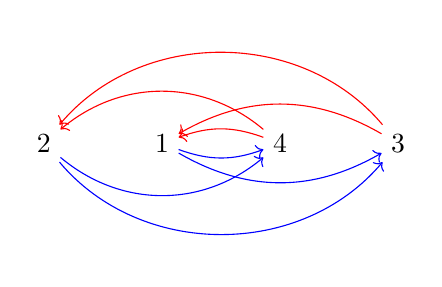
\begin{tikzpicture}[scale=1.5]
	\node (n1) at (0,0) {$2$};
	\node (n2) at (1,0) {$1$};
	\node (n3) at (2,0) {$4$};
	\node (n4) at (3,0) {$3$};

	\draw[->,color=blue] (n1) to[bend right=40] (n3);
	\draw[->,color=blue] (n1) to[bend right=50] (n4);
	\draw[->,color=blue] (n2) to[bend right=20] (n3);
	\draw[->,color=blue] (n2) to[bend right=30] (n4);

    \draw[->,color=red] (n3) to[bend right=40] (n1);
	\draw[->,color=red] (n3) to[bend right=20] (n2);
	\draw[->,color=red] (n4) to[bend right=50] (n1);
	\draw[->,color=red] (n4) to[bend right=30] (n2);


\end{tikzpicture}
\]
\end{example}

\end{frame}

\begin{frame}{The Enumeration Algorithm cont'd}

\begin{lemma}
Without even completing the {\color{red} first pass}, we can identify if $H$, $|V(H)| = n$, has more than $c = O(n)$ edges. By setting a corresponding minimum, we can enumerate all $H$ with $|V(H)| \in [b,c]$ with $O(n \log n)$ processing for each $H$.
\end{lemma}

\begin{example}
\vspace{-0.5cm}
\[
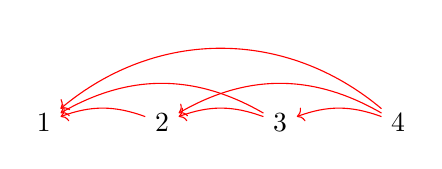
\begin{tikzpicture}[scale=1.5]
	\node (n1) at (0,0) {$1$};
	\node (n2) at (1,0) {$2$};
	\node (n3) at (2,0) {$3$};
	\node (n4) at (3,0) {$4$};

	\draw[<-,color=red] (n1) to[bend left=20] (n2);
    \draw[<-,color=red] (n1) to[bend left=30] (n3);
	\draw[<-,color=red] (n1) to[bend left=40] (n4);

	\draw[<-,color=red] (n2) to[bend left=20] (n3);
	\draw[<-,color=red] (n2) to[bend left=30] (n4);

	\draw[<-,color=red] (n3) to[bend left=20] (n4);
\end{tikzpicture}
\]
\end{example}

\end{frame}

\begin{frame}{The Enumeration Algorithm cont'd}

\begin{theorem}
Given an $n \in \mathbb{N}$, we can obtain a (small) set $H$ with
\begin{itemize}
    \item $|V(H)| = n$
    \item at least the number of edges in the target $\Grid$
    \item at most $k$ additional edges compared to the target $\Grid$
    \item degree sequence at least the degree sequence of target $\Grid$
    \item (some others)
\end{itemize}
with $O(n \log n)$ processing for each $H$.
\end{theorem}

\end{frame}

\begin{frame}{Recall: Which grids are subgraphs?}

\begin{theorem}
$\Grid_{k \times n}$ is not a subgraph of $\CGrid$ for $k > 2$. For $k = 3$, the minimum is 2 additional edges.
\end{theorem}

\begin{center}
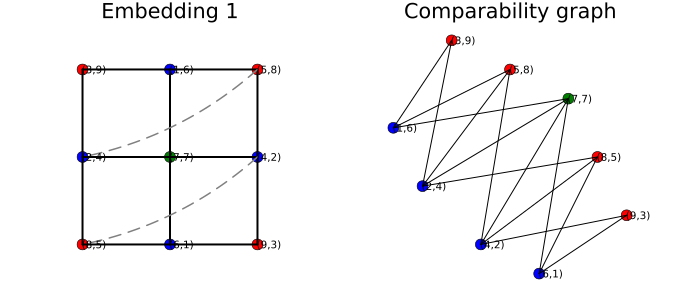
\includegraphics[width=\textwidth]{media/6-4-9-2-8-1-7-5-3.png}
\end{center}

\end{frame}



\section{The Width-3 Gadget}

\begin{frame}{The Width-3 Gadget}

\begin{definition}
The previous graph gives rise to the following width-3 gadget:
\begin{align*}
\begin{quantikz}
\lstick{$q_1$} 
    & \gate{R_z(\theta_1)} & \targ{}   & \ctrl{1} & \gate{H} & \qw \\
\lstick{$q_2$} 
    & \gate{R_z(\theta_2)} & \qw       & \ctrl{-1}& \gate{H} & \qw \\
\lstick{$q_3$} 
    & \gate{R_z(\theta_3)} & \ctrl{-2} & \qw      & \gate{H} & \qw
\end{quantikz}        
\end{align*}
\end{definition}

Question: Is this gadget universal for MBQC?

\end{frame}

% \begin{frame}{Linear Algebra Universality Algorithm}

% \begin{theorem}
% A gate set $\mathcal{G}$ is universal for $n$ qubits if it generates $SU(2^n)$, the group of $2^n \times 2^n$ unitary matrices with determinant 1.
% \end{theorem}

% \begin{theorem}[Sawicki and Karnas, 2017]
% Given a finite gate set $\mathcal{G}$, we can determine if it is universal in finite time by computing the kernel, trace, and product of some matrices and vectors.
% \end{theorem}

% \begin{problem}<2->
% The gate set $\mathcal{G}$ from the width-3 gadget is not finite, since we can choose $\theta_i \in [0, 2\pi]$.
% \end{problem}

% \end{frame}

\begin{frame}{Lie Algebra Universality Algorithm}

\begin{definition}[Matrix Exponentiation]
For any $A \in \mathbb{C}^{m \times m}$, 
\begin{align*}
    e^A = \sum_{k=0}^\infty \frac{A^k}{k!}
\end{align*}
\end{definition}

\begin{definition}<2->[Lie Algebra of $SU(2^n)$]
\begin{align*}
    \mathfrak{su}(2^n) = \{ -iH \in \mathbb{C}^{2^n \times 2^n} \mid H^\dagger = H, \text{tr}(H) = 0 \}
\end{align*}
\end{definition}

\end{frame}

\begin{frame}{Lie Algebra Universality Algorithm cont'd}

\begin{theorem}
A gate set $\mathcal{G}$ is universal for $n$ qubits if it generates $SU(2^n)$, the group of $2^n \times 2^n$ unitary matrices with determinant 1.
\end{theorem}

\begin{fact}<2->
$U \in SU(2^n)$ if and only if $U = e^{H}$ for some $H \in \mathfrak{su}(2^n)$.
\end{fact}

\begin{corollary}<2->
To show $\mathcal{G}$ is universal, it suffices to generate the Lie algebra.
\end{corollary}

\begin{fact}<3->
$H \in \mathfrak{su}(2^n)$ if and only if $H = -i \sum_{P \in \mathcal{P}_n \setminus \{I\}} \alpha_P P$ for some $\alpha_P \in \mathbb{R}$, where $\mathcal{P}_n$ is the set of Pauli matrices on $n$ qubits.
\end{fact}

\begin{corollary}<3->
The traceless Hermitian operators are exactly those that can be represented as a linear combination of Pauli operators (X, Y, Z).
\end{corollary}

\end{frame}

\begin{frame}{Lie Algebra Universality Algorithm: Cliffords}

\begin{lemma}
Denote by $G(\theta_1, \theta_2, \theta_3)$ the width-3 gadget. Then $G(0,0,0)$ is some fixed Clifford operation $C$ and $C \in \mathcal{G}$. 
\end{lemma}

\begin{lemma}<2->
If $C \in \mathcal{G}$ then $C^\dagger \in \mathcal{G}$.
\end{lemma}

\begin{proof}<3->
The Clifford group on 3 qubits is finite. Hence every element has finite order, i.e. $\exists t$ with $C^t = I$. Thus $C^\dagger = C^{t-1} \in \mathcal{G}$.
\end{proof}

\end{frame}

\begin{frame}{Lie Algebra Universality Algorithm: Addition}

\begin{fact}[Baker-Campbell-Hausdorff formula]
For $A,B \in \mathfrak{su}(2^n)$,
\begin{align*}
    e^{A} e^{B} = e^{A + B + \frac{1}{2}[A,B] + \frac{1}{12}[A,[A,B]] + \frac{1}{12}[B,[A,B]] + \cdots}
\end{align*}
where $[A,B] = AB - BA$ is the commutator of $A$ and $B$.
\end{fact}

\begin{fact}
For $A,B \in \mathfrak{su}(2^n)$,
\begin{align*}
    \lim_{k \to \infty} e^{A/k} e^{B/k} = e^{A + B}
\end{align*}
\end{fact}

\begin{corollary}
If we have $A,B$ in the Lie algebra, we can generate their sum.
\end{corollary}

\end{frame}

\begin{frame}{Lie Algebra Universality Algorithm: Commutators}

\begin{fact}
For $A,B \in \mathfrak{su}(2^n)$,
\begin{align*}
    \lim_{k \to \infty} e^{B/k} e^{A/k} e^{-B/k} e^{-A/k} = e^{[A,B]}.
\end{align*}
\end{fact}

\begin{corollary}
If we have $A,B$ in the Lie algebra, we can generate their commutator $[A,B]$.
\end{corollary}

\end{frame}

\begin{frame}{Lie Algebra Universality Algorithm: Operations}

Strategy: Start with some elements in the Lie algebra and generate more using:
\begin{itemize}
    \item Conjugation by $C$
    \item Addition
    \item Commutators
\end{itemize}

\begin{fact}<2->
We cannot generate all $|\{I,X,Y,Z\}|^3 - |(I,I,I)| = 63$ non-identity Pauli operators on $3$ qubits this way.
\end{fact}

\begin{proof}<3->
Brute force using a computer program.
\end{proof}

\end{frame}

\begin{frame}{Lie Algebra Universality Algorithm: Visual Intuition}

The $CNOT$ ``forbids us'' from generating $R_x(\theta_1)$ alone on $q_1$.
\begin{center}
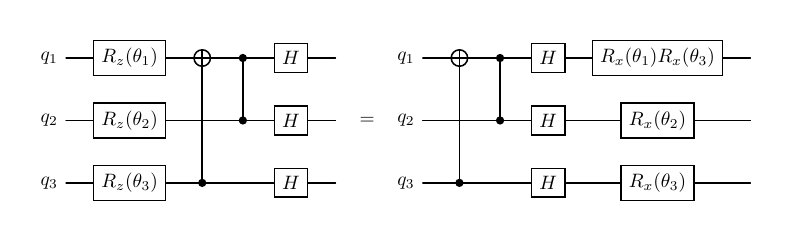
\begin{tikzpicture}[scale=0.7, transform shape]

\node (left) at (0,0) {
\begin{quantikz}
\lstick{$q_1$} 
    & \gate{R_z(\theta_1)} & \targ{}   & \ctrl{1} & \gate{H} & \qw \\
\lstick{$q_2$} 
    & \gate{R_z(\theta_2)} & \qw       & \ctrl{-1}& \gate{H} & \qw \\
\lstick{$q_3$} 
    & \gate{R_z(\theta_3)} & \ctrl{-2} & \qw      & \gate{H} & \qw
\end{quantikz}
};

\node (eq) at (3.25,0) {$=$};

\node (right) at (7,0) {
\begin{quantikz}
\lstick{$q_1$} 
    & \targ{}   & \ctrl{1} & \gate{H} & \gate{R_x(\theta_1)R_x(\theta_3)} & \qw \\
\lstick{$q_2$} 
    & \qw       & \ctrl{-1}& \gate{H} & \gate{R_x(\theta_2)} & \qw \\
\lstick{$q_3$} 
    & \ctrl{-2} & \qw      & \gate{H} & \gate{R_x(\theta_3)} & \qw
\end{quantikz}
};

\end{tikzpicture}
\end{center}

\only<2->{
Idea: ``Stitch'' this with another gadget to ``get'' $R_x(\theta_1)$ on $q_1$.
}

\end{frame}

\section{Bridging Gadgets}

\begin{frame}{Recall: Many width-3 gadgets.}

\begin{columns}[T,totalwidth=\linewidth]

\column{0.49\linewidth}
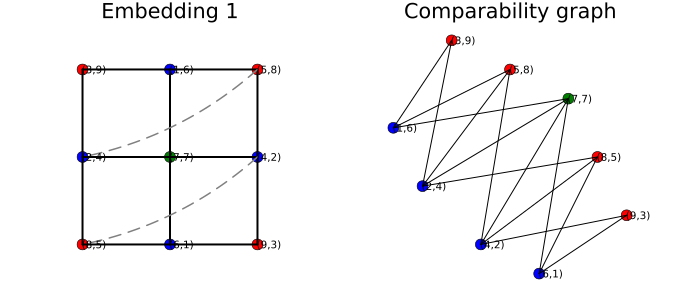
\includegraphics[width=\linewidth]{media/collage/img1}

\vspace{0.02\linewidth}

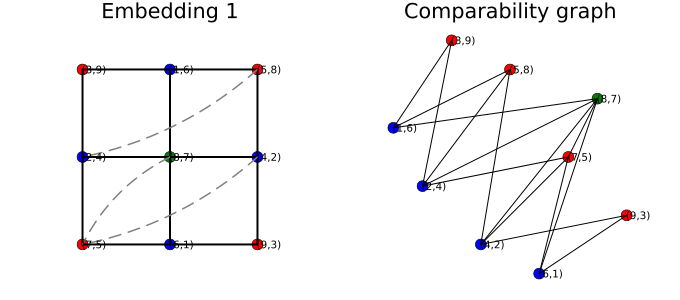
\includegraphics[width=\linewidth]{media/collage/img3}

\vspace{0.02\linewidth}

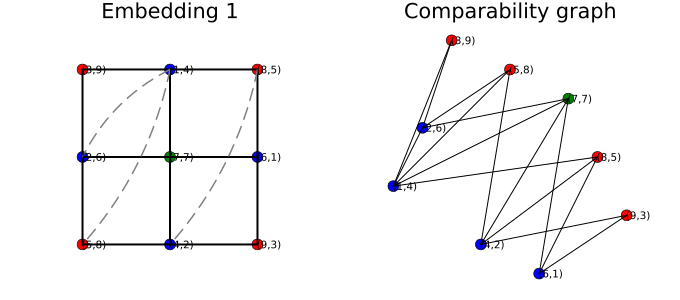
\includegraphics[width=\linewidth]{media/collage/img5}

\column{0.49\linewidth}
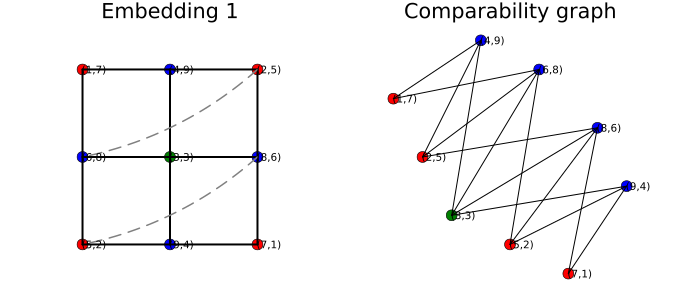
\includegraphics[width=\linewidth]{media/collage/img2}

\vspace{0.02\linewidth}

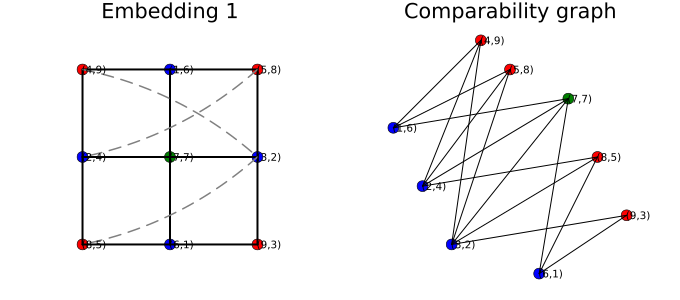
\includegraphics[width=\linewidth]{media/collage/img4}

\vspace{0.02\linewidth}

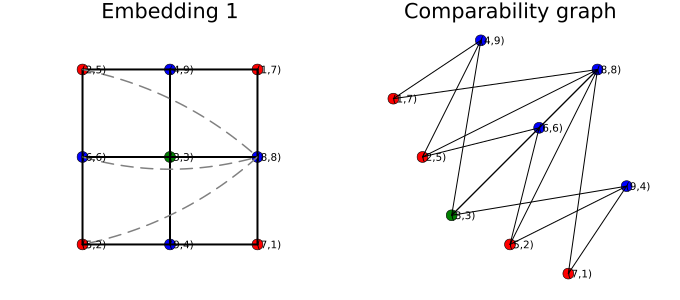
\includegraphics[width=\linewidth]{media/collage/img6}

\end{columns}

\end{frame}

\begin{frame}{Bridging Gadgets: Informal Visual Definition}

\begin{columns}[T,totalwidth=\linewidth]

\column{0.4\linewidth}

\begin{center}  
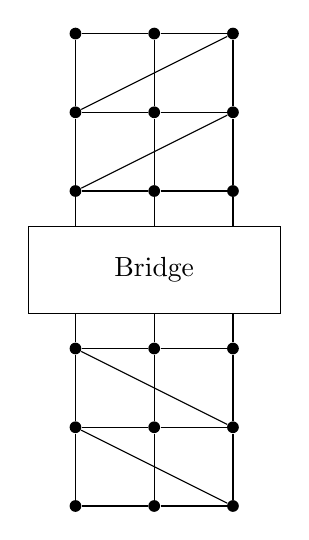
\begin{tikzpicture}[scale=1,
    dot/.style={circle, fill, inner sep=1.5pt},
    bridge/.style={draw, rectangle, minimum width=3.2cm, minimum height=1.1cm}
]

% Top 3x3 grid vertices
\foreach \x in {0,1,2}{
    \foreach \y in {0,1,2}{
        \node[dot] (T\x\y) at (\x, 4+\y) {};
    }
}

% Top grid edges
\foreach \x in {0,1,2}{
    \foreach \y in {0,1}{
        \draw (T\x\y) -- (T\x\the\numexpr\y+1\relax);
        \draw (T\y\x) -- (T\the\numexpr\y+1\relax\x);
    }
}

\draw (T00) -- (T21);
\draw (T01) -- (T22);

% Bottom 3x3 grid vertices
\foreach \x in {0,1,2}{
    \foreach \y in {0,1,2}{
        \node[dot] (B\x\y) at (\x, \y) {};
    }
}

% Bottom grid edges
\foreach \x in {0,1,2}{
    \foreach \y in {0,1}{
        \draw (B\x\y) -- (B\x\the\numexpr\y+1\relax);
        \draw (B\y\x) -- (B\the\numexpr\y+1\relax\x);
    }
}

\draw (B02) -- (B21);
\draw (B01) -- (B20);

% Bridge ellipse centered between grids
\node[bridge] (bridge) at (1,3) {Bridge};

% Define 3 attachment points on top and bottom of bridge, aligned with x=0,1,2
\foreach \x in {0,1,2}{
  \coordinate (bn\x) at (\x, 3+0.55); % near top of ellipse
  \coordinate (bs\x) at (\x, 3-0.55); % near bottom of ellipse
}

% Vertical edges from bottom row of top grid (y=4) down into bridge
\foreach \x in {0,1,2}{
  \draw (T\x0) -- (bn\x);
}

% Vertical edges from top row of bottom grid (y=2) up into bridge
\foreach \x in {0,1,2}{
  \draw (B\x2) -- (bs\x);
}

\end{tikzpicture}

\end{center}

\column{0.6\linewidth}

\begin{definition}[Informal]
A width-3 bridge of size $b \in \mathbb{N} \cup \{0\}$ adds $3b$ new vertices between two width-3 gadgets. The bridge has some $\Grid_{3 \times b}$ as a subgrid.
\end{definition}

\vspace{0.5cm}

\only<2->{
The bridge can have any number of additional edges; set $\theta = 0$ to ``ignore'' them.
}

\vspace{0.5cm}

\only<3->{
Question: Given width-3 gadgets $A$ and $B$, how can we construct a width-3 bridge of size $b$ or prove that it is impossible?
}

\end{columns}

\end{frame}

\begin{frame}{Linear Programming Bridging Algorithm}

\begin{definition}[Informal]
Given width-3 gadgets $A$ and $B$, encode each as inequalities on a linear program.
\end{definition}

\begin{example}
Suppose we are dealing with width-2 gadgets and $A$ has $\pi(A) = (2,1,4,3)$. We add conditions:
\begin{align}
    x_1 < x_2 < x_3 < x_4 \\
    y_2 < y_1 < y_4 < y_3.
\end{align}
\end{example}
\end{frame}

\begin{frame}{Linear Programming Bridging Algorithm cont'd}

\begin{lemma}[Informal]
We can add additional inequalities to a linear program encoding $A$ to also encode $B$ and any bridge vertices.
\end{lemma}

\begin{theorem}
Fix a bridge size $b$. If the corresponding linear program is infeasible, then there is no bridge of size $b$ between $A$ and $B$.
\end{theorem}

\begin{fact}<2->
There exists no bridge of size $b < 4$ between any two width-3 gadgets $A$, $B$, where each gadget has at most 3 additional edges compared to $\Grid_{3 \times 3}$.
\end{fact}

\begin{proof}<3->
Brute force every linear program encoding of ordered pairs of gadgets $A,B$ with at most 3 additional edges.
\end{proof}

\end{frame}

\section{Conjectures}

\begin{frame}{Resolution?}

\begin{conjecture}
$\CGrid$ is not a universal resource for MBQC.
\end{conjecture}

\begin{justification}<2->
Considering gadgets with more additional edges is unlikely to help get $R_z(\theta_1)$ on $q_1$. 
\end{justification}

\only<2->{%
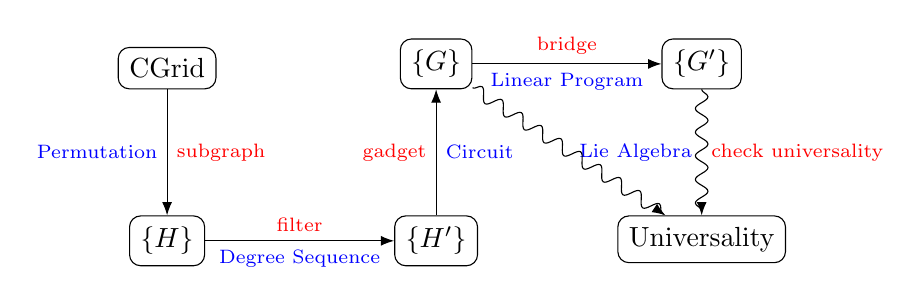
\begin{tikzpicture}[
>=Latex,
node distance=16mm and 24mm,
box/.style={draw, rounded corners, inner sep=4pt, align=center},
lab/.style={font=\scriptsize}
]

\node[box] (cgrid) {CGrid};
\node[box, below=of cgrid] (H) {$\{H\}$};
\node[box, right=of H] (Hp) {$\{H'\}$};
\node[box, above=of Hp] (G) {$\{G\}$};
\node[box, right=of G] (bridge) {$\{G'\}$};
\node[box, below=of bridge] (yesno) {Universality};

\draw[->] (cgrid) -- (H)
node[midway, right, lab]{\color{red} subgraph}
node[midway, left, lab]{\color{blue} Permutation};

\draw[->] (H) -- (Hp)
node[midway, above, lab]{\color{red} filter}
node[midway, below, lab]{\color{blue} Degree Sequence};

\draw[->] (Hp) -- (G)
node[midway, left, lab]{\color{red} gadget}
node[midway, right, lab]{\color{blue} Circuit};

\draw[->] (G) -- (bridge)
node[midway, above, lab]{\color{red} bridge}
node[midway, below, lab]{\color{blue} Linear Program};

\draw[->, decorate, decoration={snake, amplitude=0.8mm, segment length=3mm}]
(bridge) -- (yesno)
node[midway, right, lab]{\color{red} check universality}
node[midway, left, lab]{\color{blue} Lie Algebra};

\draw[->, decorate, decoration={snake, amplitude=0.8mm, segment length=3mm}] 
(G) -- (yesno);

\end{tikzpicture}
}

\end{frame}

\section{Motivation for Comparability Grids}

\begin{frame}{Why Care about Comparability Grids?}

\begin{theorem}[Maarten Van den Nest et al, 2006]
Let $\Psi$ be a family of resource states, and $\ket\phi, \ket{\phi'}$ arbitrary states with the same number of qubits. Let $E: \ket\phi \to \mathbb{R}$ be a function that satisfies the following properties:
\begin{enumerate}
    \item $E(\ket\phi) \geq E(\ket{\phi'})$ whenever $\ket\phi \geq_{\LOCC} \ket{\phi'}$;
    \item $\sup_{\ket\phi} E(\ket\phi) > \sup_{\ket\psi \in \Psi} E(\ket\psi)$. 
\end{enumerate}
Then $\Psi$ cannot be a universal resource.
\end{theorem}

\begin{theorem}<2->
$\CGrid$s have unbounded rank width (and so do grid graphs).
\end{theorem}

\begin{corollary}<3->   
If $\CGrid$ is not a universal resource, then unbounded rank width is not sufficient for universality.
\end{corollary}

\end{frame}

\end{document}